\documentclass[a4paper,11pt,dvipdfmx]{ujarticle}
% パッケージ
\usepackage{graphicx}
\usepackage{url}
% レイアウト指定を記述したファイルの読み込み
\input{layout}

% タイトルと氏名を変更せよ.
\title{日本におけるデジタル化の状況}
\author{G584232025 臼井 七海}

\begin{document}

\maketitle %ここにタイトルが入る

% ここから本文
% 節見出し: \section{}
% を使う
\section{ブロードバンドの整備状況}

% 本文(1)
%  参考文献の参照: \cite{}
%  図番号の参照: \ref{}
% を使う
% 文献データベースのキーワードは oecd と imd
% になっている.
OECDによるブロードバンド回線の普及に関する調査\cite{oecd}によると、
図\ref{fig:加入者数}に示すように、
日本における100人あたりの光ファイバー回線の加入者数は 29.0 で、韓国、スウェーデン、ノルウェーに続いて第4位になっている。

% 図の挿入
% \includegraphics{}
% を
% \begin{figure}[htbp]
% \end{figure}
% で囲み
% \caption{}
% で図のタイトルを入れる.
% \label{}
% を使って図番号が参照できるようにする
% また,
% \centering
% で図が中央に来るようにする
\begin{figure}[htbp]
    \centering
    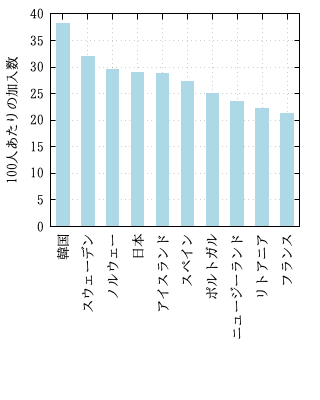
\includegraphics{graph.png}
    \caption{光ファイバー回線の加入者数(100人あたり)}\label{fig:加入者数}
\end{figure}

% ーーー
% 節見出し(2)
\section{デジタル競争力ランキング}

% 本文(2)
国際経営開発研究所(IMD)の調査\cite{imd}によると、
日本のデジタル競争力のランキングは表\ref{tbl:ランキング}に示すように、
調査対象の64カ国中、総合で28位、技術分野で30位となっている。

% 表の挿入
% \begin{tabular}
% \end{tabular}    
% による表の記述を 
% \begin{table}[htbp]
% \end{table}
% で囲み
% \caption{}
% で表のタイトルを入れる.
% \label{}
% を使って表番号が参照できるようにする
% また,
% \centering
% で表が中央に来るようにする
\begin{table}[htbp]
    \centering
    \caption{デジタル競争力ランキング(64カ国中)}
    \label{tbl:ランキング}

    \begin{tabular}{|c|c|c|}\hline
        国 & 総合 & 技術 \\
        \hline
        米国 & 1位 & 4位 \\
        \hline
        香港 & 2位 & 10位 \\
        \hline
        スウェーデン & 3位 & 8位 \\
        \hline
        デンマーク & 4位 & 2位 \\
        \hline
        シンガポール & 5位 & 3位 \\
        \hline
        \hline
        韓国 & 12位 & 13位 \\
        \hline
        中国 & 15位 & 20位 \\
        \hline
        \hline
        日本 & 28位 & 30位 \\
        \hline
    \end{tabular}
\end{table}

% ーーー
% 見出し(3)
% 考察
%
% \begin{itemize}
% \end{itemize}
% を使って箇条書きで記述する
\section{考察}

\begin{itemize}
    \item 光ファイバー回線の加入者数は韓国が1位である
    \begin{itemize}
        \item デジタル競争力のランキングが総合12位、技術13位であることから光ファイバーの普及率が高くても競争力が高いとは限らない
    \end{itemize}
    \item 韓国、スウェーデン、日本以外の国は光ファイバー回線の加入者数上位10位に入っていない
    \item デジタル競争力ランキングより、総合と技術のランキングの差が一番大きい国は香港である
    \begin{itemize}
        \item 今後、技術力により総合ランキングの順位が低下する可能性がある
        \item 差が小さい国の中には普及率によって総合順位が上がっている国があるため、技術力向上により総合力が上がる可能性がある
    \end{itemize}
    \item 日本は光ファイバーの普及率4位、デジタル競争ランキングは総合28位、技術30位である
    \begin{itemize}
        \item 普及率のランキングは高いが他2つのランキングは低いため、技術力が向上すれば総合ランキングが上がる可能性がある
    \end{itemize}
\end{itemize}

% ここに参考文献が入る
%
\bibliographystyle{junsrt}
\bibliography{exercise.bib}

\end{document}